%!TEX root = ../../thesis.tex
\section[Accelerated computation of PDE-like systems]{Accelerated computation of PDE-like systems using Matrix Differentials}
\label{sec: chap2 section header}
Due to the partial differential nature of soft robots, obtaining a closed-form expression for the projected Lagrangian model in \eqref{eq:C2:dynamic_model} can become notoriously long and complex (especially for multi-link systems). The origin of this problem stems from the integrands of inertia matrix $\mat{M}(\q)$ in \eqref{eq:C2:kinetic_energy} and Coriolis forces $\mat{C}(\q,\dq)$ in \eqref{eq:C2:coriolis}; which become highly nonlinear and therefore difficult to calculate a-priori. As a result, solving the forward dynamics using traditional solvers often deteriorates the real-time performance, and in turn its usability for closed-loop control. Inspired by Boyer et al. \cite{Boyer2021}) and Godage et al. 
\cite{Godage2016}), instead of finding an exact solution to the dynamic entries $\mat{M}(\q)$, $\mat{C}(\q,\dq)$ and $\mat{f}\!\grav(\q)$, let us introduce a similar reduced-order integration scheme that produces an approximate of the dynamic model \eqref{eq:C2:dynamic_model}. Yet, \editl instead of using an inverse Newton-Euler algorithm (i.e., Featherstone algorithm \cite{Spong2006}) \editr in which the Lagrangian entries are built column-wise, we propose an explicit integration scheme that efficiently computes all Lagrangian entities in parallel through a so-called Matrix-Differential Equation (MDE).

The idea here is to replace all necessary spatial integrations required for the Lagrangian entities with an equivalent Matrix-Differential Equation of the form:
%
\begin{equation}
\frac{\p \vec{Z}}{\p \sigma} = \mat{F}(\vec{Z},\sigma), \label{eq:C2:MDE}
\end{equation}
%
where $\vec{Z}(\cdot,\sigma)$ is a matrix-valued function composed of the necessary elements for the forward kinematics and forward dynamics, and $\vec{F}(\vec{Z},\sigma)$ a matrix-valued flow function that describes the spatial evolution of $\vec{Z}$. Then, by choosing the appropriate initial condition for $\vec{Z}(\cdot,\sigma = 0) = \vec{Z}_0$ and numerically solving \eqref{eq:C2:MDE} over a finite horizon $\Xs$, we can retrieve an approximate of the Lagrangian model in
\eqref{eq:C2:dynamic_model} by extracting the necessary elements from the solution $\vec{Z}(\cdot,L)$.

Before describing the MDE, let us first introduce two intermediate matrices related to the computation of the manipulator Jacobian and its time-derivative, namely:
%
\begin{align}
\frac{\p \mat{B}_1}{\p \sigma} &= \Ad_{\gB(\cdot,\sigma)}\, \mat{J}^\star \vec{\Theta}(\sigma) \\[0.5em]
\frac{\p \mat{B}_2}{\p \sigma} &= \Ad_{\gB(\cdot,\sigma)}\ad_{\etaB(\cdot,\sigma)}\, \mat{J}^\star \ThetaB(\sigma)
\end{align}
%
such that they satisfy $\vec{J} \dq = {\Ad_{\mat{g}}}^{-1} \vec{B}_1 \dq$ and $\,\dot{\!\vec{J}} \dq = {\Ad_{\mat{g}}}^{-1} \mat{B}_2 \dq$.
Given the expressions above, we can now include a partial computation Jacobians into the MDE. By collecting all the differential relation for the forward kinematics \eqref{eq:C2:change_phi}, \eqref{eq:C2:change_p}, \eqref{eq:C2:vel_cont} and forward dynamics \eqref{eq:C2:kinetic_energy}, \eqref{eq:C2:coriolis} and
\eqref{eq:C2:potential_energy_grav}, we can assign a flow function
$\mat{F}:= \text{blkdiag}\left(\mat{F}_1,\mat{F}_2 \right)$
composed of two matrices:
%
\begin{align}
\mat{F}_1 & = \begin{pmatrix}
\begin{matrix} \PhiB \vec{\Gamma}^\times & \PhiB \vec{U} \\[0.35em] \vec{0}_{3\times3} & \vec{0}_3 \end{matrix}
\;\; \vrule\; & \Ad_{\gB} \JB^\star\mat{S} &\vrule\;\; \Ad_{\gB} \ad_{\etaB} \JB^\star \mat{S}
\end{pmatrix}, \\[0.75em]
\mat{F}_2 & = \begin{pmatrix}
\dfrac{\p \mat{M}}{\p \sigma} & \dfrac{\p \mat{C}}{\p \sigma} & \dfrac{\p \vec{f}\!\grav}{\p \sigma} \end{pmatrix},
\end{align}
%s
in which the differential form of the dynamic entities $\mat{M}(\q)$, $\mat{C}(\q,\dq)$, and $\vec{f}\!\grav(\q)$ of the Lagrangian model are given by
%
\begin{align}
\dfrac{\p \mat{M}}{\p \sigma} & = (\Ad_{\gB}\inv \mat{B}_1)^\top \ten{M} (\Ad_{\gB}\inv \mat{B}_1), \\[0.6em]
\dfrac{\p \mat{C}}{\p \sigma} & = (\Ad_{\gB}\inv \mat{B}_1)^\top \left[\ten{C}_\etaB (\Ad_{\gB}\inv \mat{B}_1) + \ten{M} (\Ad_{\gB}\inv \mat{B}_2) \right], \\[0.6em]
\dfrac{\p \vec{f}\!\grav}{\p \sigma} & = (\floor{\mat{B}_{1}}_3)^\top \rho_0\, \vec{a}_g,
\end{align}
%
% \begin{figure}[!t]
%   \vspace{-0.6mm}
%   \centering
%    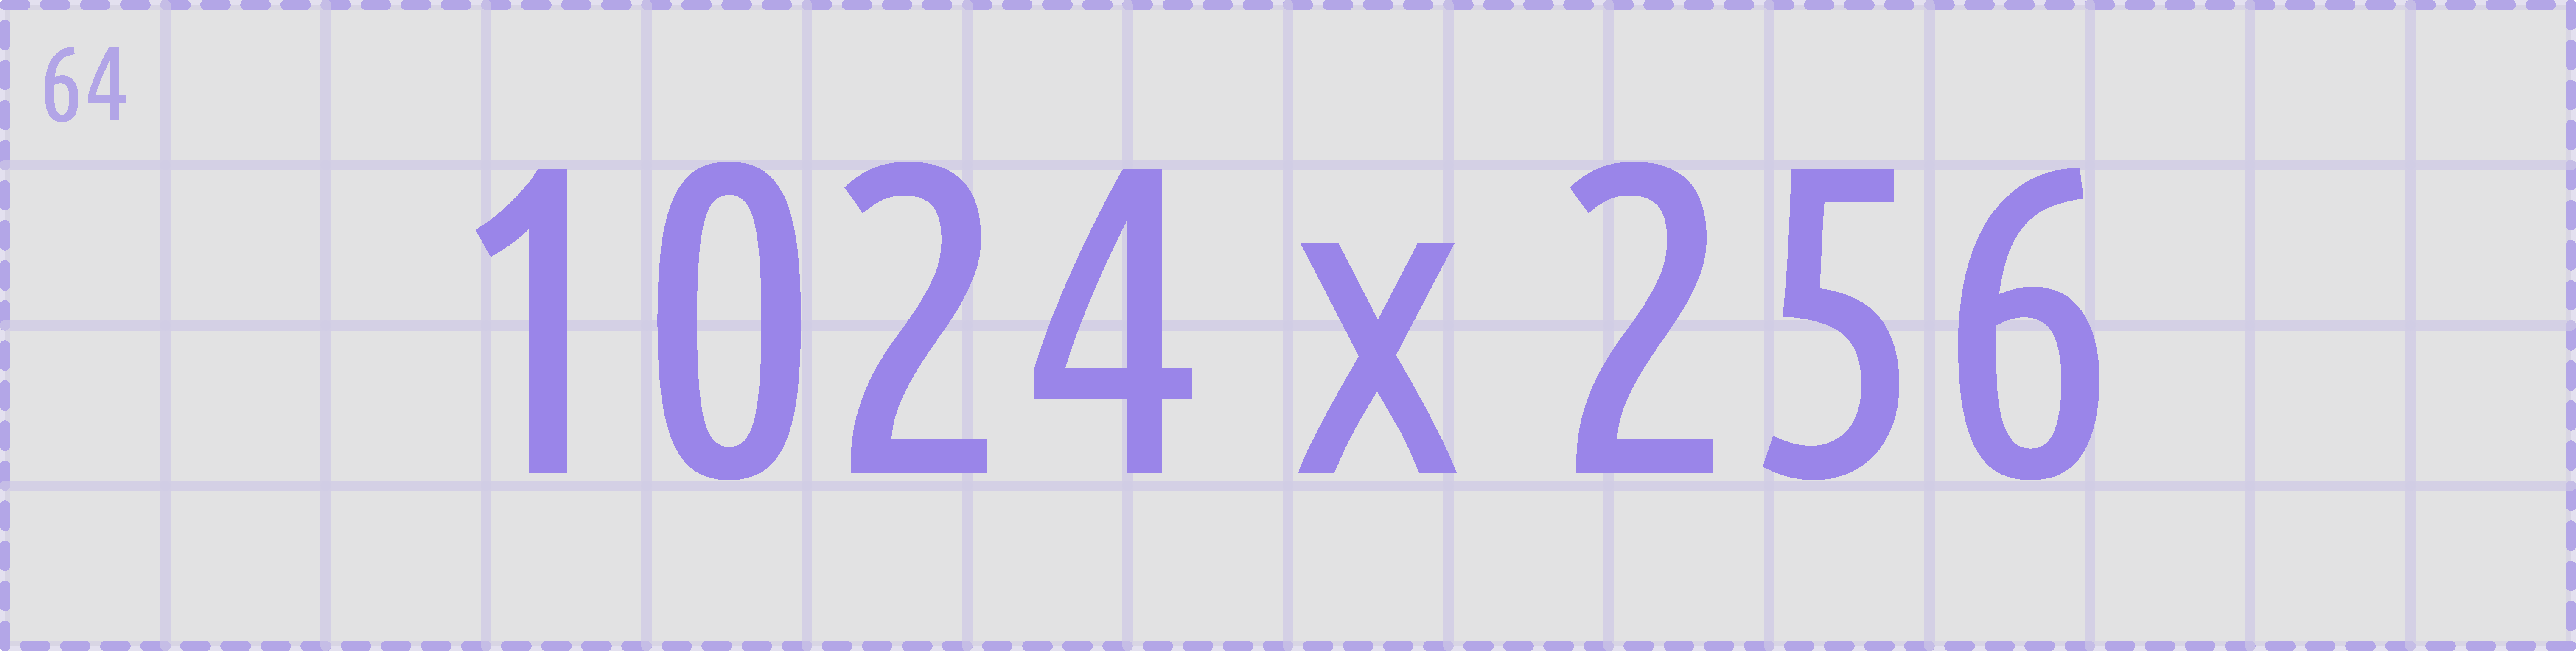
\includegraphics[width = 0.99\textwidth]{fig_1024x256.pdf}
%   \caption{Diagram of the efficient Matrix-Differential solver to compute the unknown Lagrangian entries in the model \eqref{eq:C2:dynamic_model}}
%   \vspace{-0.1cm}
%   \label{fig:C2:EX1:strain_ref}
% \end{figure}
% \begin{figure}[!t]
%  \vspace{-3mm}
%   \centering
%   \def\svgwidth{0.9\linewidth}
%   \input{./3_chapters/2_chapter/img/fig_C2_solver_diagram.pdf_tex}
%   \vspace{-0.25cm}
%   \caption{bla}
%   \vspace{-0.1cm}
%   \label{fig:C2:stiffness_model}
% \end{figure}
%
We wish to stress that $\mat{F}_1$ collects all elements related to the forward kinematics, whereas $\mat{F}_2$ contains the dynamic entities related to the Lagrangian model. Following the spatial Matrix-Differential equation in \eqref{eq:C2:MDE} above, its solution will be a matrix $\mat{Z} := \text{blkdiag}\left( \mat{Z}_1, \mat{Z}_2 \right)$ composed of two state matrices $\mat{Z}_1$ and $\mat{Z}_2$:
%
\begin{align}
\mat{Z}_1(\sigma,\q,\dq) & := \begin{pmatrix}
\begin{matrix}
\PhiB  & \gammaB \\ 0_{3\times3} &  0_{3}
\end{matrix} \;\; \vrule & \!\mat{B}_1 & \vrule & \!\mat{B}_2 \;\;\;
 \end{pmatrix}, \\[0.5em]
\mat{Z}_2(\sigma,\q,\dq) & := \begin{pmatrix} \mat{M} & \mat{C} & \mat{f}\!\grav \end{pmatrix},
\end{align}
%
Such a set of Matrix-Differentials as in \eqref{eq:C2:MDE} are not supported natively by standard ODE solvers. Therefore, an explicit second-order Runge-Kutta solver for MDEs is developed such that efficiently computes the evolution of the state matrix $\mat{Z}$ along $\Xs = [0,L]$. The numerical solver is written in \matlab \texttt{2021a} and it can be found in the public repository of \sorotoki (see implementation at \cite{SorotokiCode}).

As for state trajectories along the temporal regime $\mathbb{T} = [0,T]$, an implicit trapezoidal integration scheme is proposed to solve the approximated continuum dynamics, which are generally less conservative on discretization to preserve numerical stability. Here implicit schemes are favored over the explicit scheme since a coarser time integration can significantly increase real-time performance. In addition, to further boost the performance of the temporal integration, a cost-effective approximation of the Hessian is introduced. For more detail on the temporal integration scheme of the solver can be found in Appendix \ref{app:C2:timeint}
